% template by Chuck Anderson
% www.cs.colostate.edu/~anderson/cs410/proposal.tex

\documentclass{article}
\usepackage{pgf}
\usepackage{tikz}

% Set margins to 1 inch
\setlength{\oddsidemargin}{0in}
\setlength{\evensidemargin}{0in}
\setlength{\headheight}{12pt}
\setlength{\headsep}{42pt}
\setlength{\topmargin}{-54pt}
\setlength{\textwidth}{6.5in}
\setlength{\textheight}{9in}
\usepackage{graphicx}

\begin{document}

\title{Secure GPU Computing Over LAN}
\author{Attique Dawood}
\maketitle

\section{GPU Computing}

Graphics processing units (GPU) have evolved over the last half a decade from a graphics--only processor to a general purpose computing device. General purpose GPU (GPGPU) computing is the use of GPUs for engineering and scientific computations. The two major manufacturers of GPUs are nVidia and AMD/ATi. Both offer tools and APIs to program their GPUs.

GPUs nowdays are capable of performing teraflops of computations. The GPGPU computing model is to have CPU work in conjunction with GPU. The computationally intensive part is run on GPU while the rest of the program executes on CPU. Figure~\ref{nVidiaGPGPUfig} illustrates this.

\begin{figure}[here]
%\centerline{\includegraphics[]{GPGPU}}
\centering
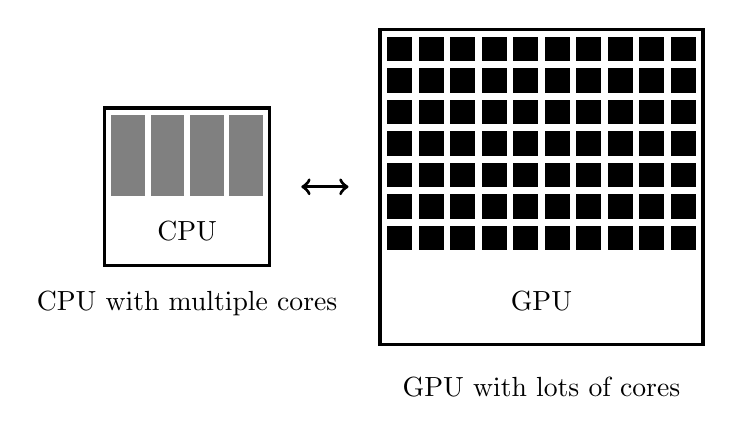
\begin{tikzpicture}
	\draw[very thick] (0cm, 0cm) rectangle (2.1cm, 2cm);
	\foreach \x in {0.1cm,0.6cm,1.1cm, 1.6cm}
		\filldraw[gray, thick] (\x, 0.9cm) rectangle (\x+0.4cm, 1.9cm);
	\coordinate [label=above:CPU] (CPU) at (1.05cm,0.2cm);
	\coordinate [label=below:CPU with multiple cores] (Multi Core CPU) at (1.05cm,-0.2cm);
	
	\draw[very thick, <->] (2.5cm, 1cm) -- (3.1cm, 1cm);
	
	\draw[very thick] (3.5cm, -1cm) rectangle (7.6cm, 3cm);
		\foreach \x in {3.6cm,4cm,4.4cm,4.8cm,5.2cm,5.6cm,6cm,6.4cm,6.8cm,7.2cm}
			\foreach \y in {0.2cm,0.6cm,1cm,1.4cm,1.8cm,2.2cm,2.6cm}
				\filldraw (\x, \y) rectangle (\x+0.3cm, \y+.3cm);
	\coordinate [label=above:GPU] (GPU) at (5.55cm,-0.7cm);
	\coordinate [label=below:GPU with lots of cores] (Multi Core GPU) at (5.55cm,-1.3cm);		
\end{tikzpicture}
\caption{GPGPU Computing.}
\label{nVidiaGPGPUfig}
\end{figure}

\begin{thebibliography}{2}

\bibitem{nVidiaGPGPU}
http://www.nvidia.com/object/GPU\_Computing.html

\bibitem{GPGPUwiki}
http://en.wikipedia.org/wiki/GPGPU

\end{thebibliography}

\end{document}




